\documentclass[a4paper,class=article,border=10pt,tikz]{standalone}
\usepackage{tikz}
\usetikzlibrary{snakes,calc,positioning,patterns,angles,quotes,decorations.pathmorphing,decorations.markings,through}
\usetikzlibrary{arrows,decorations,decorations.text}
\usepackage{rotating}
\usetikzlibrary{arrows,decorations,decorations.text}
\usetikzlibrary{patterns.meta,math}




\usepackage{siunitx}

\begin{document}

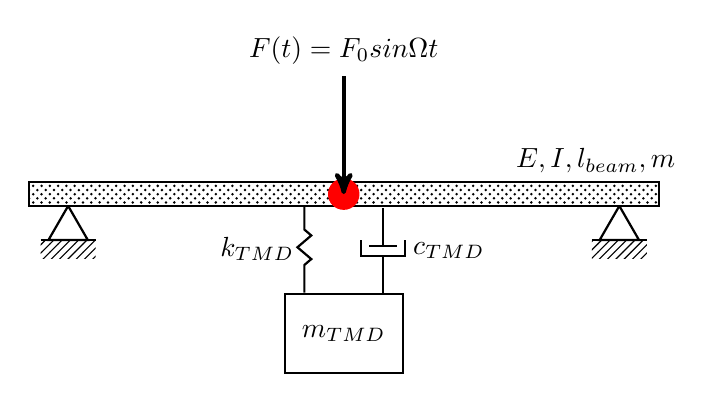
\begin{tikzpicture}

    \tikzstyle{ground}=[fill,pattern=north east lines,draw=none,minimum width=0.75cm,minimum height=0.3cm]
     \tikzstyle{close}=[draw=none,minimum width=0.75cm,minimum height=0.3cm]
    \tikzstyle{spring}=[thick,decorate,decoration={zigzag,pre length=0.3cm,post length=0.3cm,segment length=0.3cm}]
    \tikzstyle{force}=[>=stealth',ultra thick]
\tikzstyle{damper}=[thick,decoration={markings,  
  mark connection node=dmp,
  mark=at position 0.5 with 
  {
    \node (dmp) [thick,inner sep=0pt,transform shape,rotate=-90,minimum width=15pt,minimum height=3pt,draw=none] {};
    \draw [thick] ($(dmp.north east)+(2pt,0)$) -- (dmp.south east) -- (dmp.south west) -- ($(dmp.north west)+(2pt,0)$);
    \draw [thick] ($(dmp.north)+(0,-5pt)$) -- ($(dmp.north)+(0,5pt)$);
  }
}, decorate]


      \coordinate (origo) at (0,0);




    \node (part1) [draw,pattern=crosshatch dots,outer sep=0pt,thick,minimum width=8cm, minimum height=0.3cm,anchor=east,label={right,above=:{}}] at (origo){};
    \node (p1_label) at ($(part1) + (3.2,0.7)$) [below] {$E, I, l_{beam}, m$};


\draw [thick] ([xshift=0.5cm,yshift=-0.0cm]part1.south west)--++ (-60:0.5)--++(-0.5,0) node (support_end){}--++ (60:0.5);
\node (fixed_support) [ground,outer sep=0pt,thick,anchor=north west,xshift=-0.1cm,yshift=0cm,minimum height=0.1cm ,minimum width=0.7cm]  at (support_end) {};

\draw [thick] (fixed_support.north west) -- (fixed_support.north east);
% % 
\draw [thick] ([xshift=-0.5cm,yshift=-0cm]part1.south east) --++ (-60:0.5) --++(-0.5,0)  node (support_start) {}  --++ (60:0.5);
% % 
\node (floating_support) [ground,outer sep=0pt,thick,anchor=north west,xshift=-0.1cm,yshift=0cm,minimum height=0.1cm ,minimum width=0.7cm]  at (support_start) {};
% % 
\draw [thick] (floating_support.north west) -- (floating_support.north east);

\fill [red] (part1.center) circle (0.2);

\draw [thick] ([yshift=-0.1cm]origo) -- ([yshift=0.1cm]origo);

\draw [color=black,force,<-]  (part1.center) node [above=1.5cm] (R){$F(t)=F_0sin\Omega t$}     -- ++(0cm,1.5cm) ;

\draw [spring] ([xshift=-0.5cm]part1.south)  node[] (center_spring){}  --++ (0cm,-1.1cm) node[midway,left] {$k_{TMD}$};

\node (mass) [draw,outer sep=0pt,thick,minimum width=1.5cm, minimum height=1cm, label={center:$m_{TMD}$}] at (center_spring.south)[xshift=0.5cm,yshift=-1.49cm] {};

\draw [damper] ([xshift=0.5cm]mass.north)  node[] (center_damper){}  --++ (0cm,1.1cm) node[midway,right,xshift=0.25cm] {$c_{TMD}$};

\end{tikzpicture}


\end{document}
